\documentclass[11pt]{article}
\usepackage[utf8]{inputenc}	% Para caracteres en español
\usepackage{amsmath,amsthm,amsfonts,amssymb,amscd}
\usepackage{multirow,booktabs}
\usepackage[table]{xcolor}
\usepackage{fullpage}
\usepackage[export]{adjustbox}
\usepackage{lastpage}
\usepackage{enumitem}
\usepackage{fancyhdr}
\usepackage{mathrsfs}
\usepackage{wrapfig}
\usepackage{setspace}
\usepackage{calc}
\usepackage{multicol}
\usepackage{cancel}
\usepackage[retainorgcmds]{IEEEtrantools}
\usepackage[margin=3cm]{geometry}
\usepackage{amsmath}
\usepackage{graphicx}
\newlength{\tabcont}
\setlength{\parindent}{0.0in}
\setlength{\parskip}{0.05in}
\usepackage{empheq}
\usepackage{framed}
\usepackage[most]{tcolorbox}
\usepackage{xcolor}
\usepackage{import}
\usepackage{xifthen}
\usepackage{pdfpages}
\usepackage{transparent}
\colorlet{shadecolor}{orange!15}
\parindent 0in
\parskip 12pt
\geometry{margin=1in, headsep=0.25in}
\theoremstyle{definition}
\newtheorem{defn}{Definition}
\newtheorem{reg}{Rule}
\newtheorem{exer}{Exercise}
\newtheorem{sln}{Solution}
\newtheorem{note}{Note}
\begin{document}
\setcounter{section}{0}
\title{}

\thispagestyle{empty}
\begin{center}
\textsc{\LARGE German University in Cairo}\\[1.0cm]
{\LARGE \bf Lecture 1}\\ [0.5cm]
{\large \bf Strength of Materials I (ENME 401)}\\ [0.5cm]
Spring 2021
\end{center}
\tableofcontents
\newcommand{\incfig}[2][1]{%
    \def\svgwidth{#1\columnwidth}
    \import{./figures/}{#2.pdf_tex}
}
\section*{Learning objectives:}
\begin{itemize}

\item know the concept of stress in design 
\item the difference between all types of stresses

\end{itemize}

\section{Concept of Stress}
\begin{exer}
	\textbf{Analyze } Vs \textbf{Design}  in problems

\end{exer}
The main goal of our study in this course is to avoid deformation, we can do this in two ways either analyzing or desiging :) 
\begin{defn}
Strength of materials
\end{defn}
it's the branch of applied mechanics that deals with the behavior of elastic bodies subjected to various tyoes of loading.\\
\textbf{Bodies} under investigation represent the components of a machine or a structure.\\
\textbf{Coponents}
\begin{itemize}

\item \textbf{Bars} Axial Loading 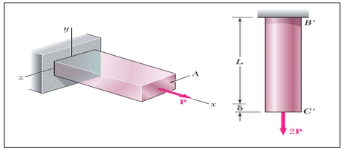
\includegraphics[scale=0.5]{figures/2021-03-30_21-09.png}
\item \textbf{Shafts} Torsion 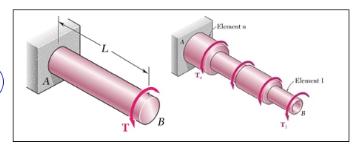
\includegraphics[scale=0.5]{figures/2021-03-30_21-09_1.png}
\item \textbf{Beams} Bending 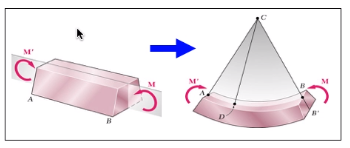
\includegraphics[scale=0.5]{figures/2021-03-30_21-09_2.png}
\item \textbf{Columns} Compression-buckling (Strength II)
\end{itemize}
once you have a force, you have \textbf{stress}, and once you have a stress you have deformation. That \textbf{deformation} causes a \textbf{strain} .
\subsection{Statics}
in statics all our attention was directed upon finding forces only, we didn't care about the \textbf{thickness}  of the cord, the \textbf{material}  it was maded from, the \textbf{dimesnions}  of it.\\
in order for the boom,rod and juncions to handle the forces and loads given and not deform, we have to study the stress on them.
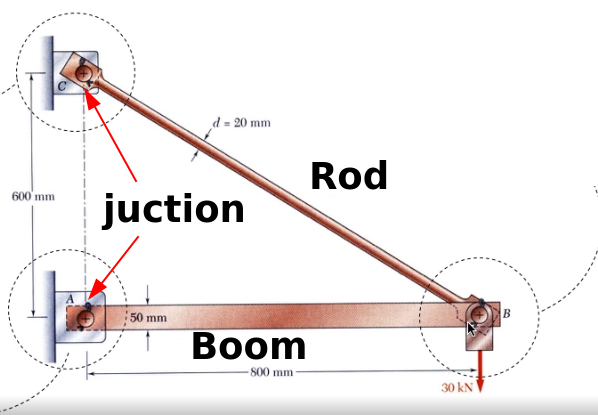
\includegraphics[scale=0.5]{figures/2021-03-30_21-41.png}
\subsection*{Design and Analyze}
To \textbf{design} is to take the load and make a structure that handels such a load, so the structure doesn't exist yet ! \\ and to \textbf{analyze} is to check if the dimesnions and the material that already exist is able to handle that load ? if not we get the maximum load we can bear.
\begin{reg}
	To solve any \textbf{strength}  problem you have to solve the \textbf{statics}  first!
\end{reg}
\begin{equation}
	Stress = \sigma = \frac{P}{A} = N/m^2 (or Pa) 
\end{equation}
Solving the previous problem using statics we will find that $F_{AB} = 40kN$ (Compression) and $F_{BC}=50kN$ (Tension). Now let's assume it's made of steel and let's calculate the stress
\begin{equation}
	\sigma_{BC} = \frac{P}{A} = \frac{50*10^2}{314*10^{-6}} = 159 MPa.  
\end{equation}
we know from the material properties for steel theat the allowable strees is $\sigma_{all} = 165MPa$ and since $\sigma_{BC} <= \sigma_{all}$ thus the strength of memeber $BC$ is adequate (safe).
\begin{note}
	if $\sigma_{member}=\sigma_{all} $ that's a risky region
\end{note}
\subsection{Stress types}
\begin{itemize}

	\item Normal stress (force prependicular to the cross sectional area)
	\item Shear Stress (force parallel to the cross-sectional area)
		\begin{itemize}
		
		\item single shear
		\item double shear
		
		\end{itemize}
	\item Bearing Stress ()

\end{itemize}
\subsection{Normal Stress}
when the resultant of the internal forces for an \textbf{axially loaded} member is \textbf{normal} to a section cut prependicular to the member axis.
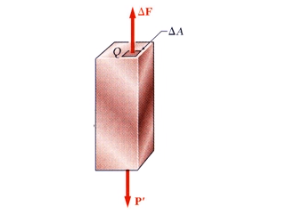
\includegraphics[scale=0.5]{figures/2021-03-30_22-07.png}
the force intensity (force per unit area) on that section is defined as the normal stress.
\begin{equation}
	\sigma = lim_{\Delta A \to 0} \frac{\Delta F}{\Delta A}  = \sigma_{ave} = \frac{P}{A} (average) 
\end{equation}
\begin{note}
Why average ? Because the stress is not unifromly distributed across the cross-sectional area.
\end{note}
\subsection{Types of Normal Load}
\begin{itemize}

	\item \textbf{Centric} $\to$ when the line of action of the resultant of the internal forces passes through the centroid of the section. \begin{reg}
	Uniform distribution of stress is possible in this case; where the concentraded loads on the end sections of two-force members are applied at the section centroids. 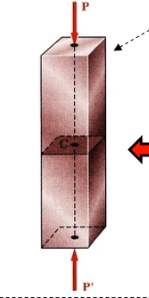
\includegraphics[scale=0.5]{figures/2021-03-30_22-21.png}
	\end{reg}
\item \textbf{Eccentric} $\to$ this is when the two-force member is \textbf{eccentrically loaded} then the resultant of the streess distibution in a section must yiels in an axial force and a moment. This moment causes \textbf{bending}  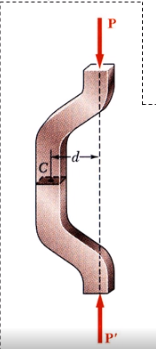
\includegraphics[scale=0.5]{figures/2021-03-30_22-22.png} 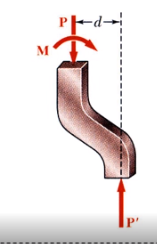
\includegraphics[scale=0.5]{figures/2021-03-30_22-22_1.png}
\begin{reg}
Eccentrically loaded members' stress cannot be uniform neither symmetric.
\end{reg}
\end{itemize}
\begin{exer}
A short post constructed from a hollow circular 
tube of aluminum supports a compressive load 
of 115 kN. The outer and inner diameters of 
the tube are do= 115 mm and di= 100 mm, 
respectively.\\
Determine the compressive stress in the post 

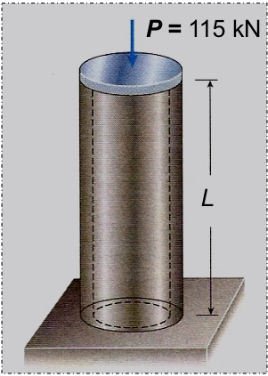
\includegraphics[scale=0.5]{figures/2021-03-30_22-24.png} 
\end{exer}
\begin{sln}
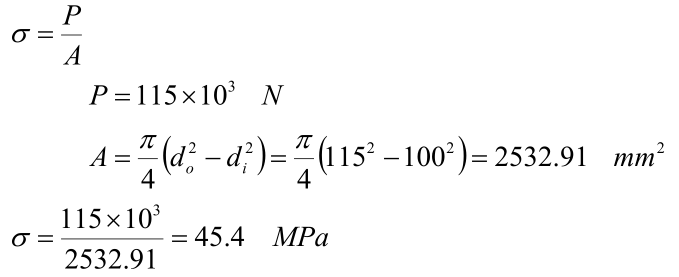
\includegraphics[scale=0.5]{figures/2021-03-30_22-38.png}
\end{sln}
\begin{exer}
Two solid cylindrical rods AB and BC 
are welded together at B and loaded 
as shown. Determine the average 
stress at the midsection of: (a) rod 
AB, (b) rod BC.
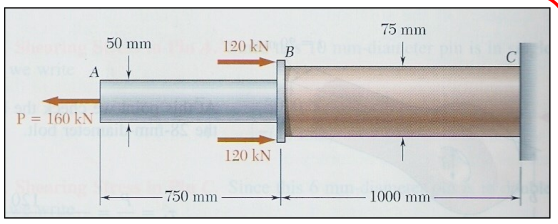
\includegraphics[scale=0.5]{figures/2021-03-30_22-37.png}
\end{exer}
\begin{sln}
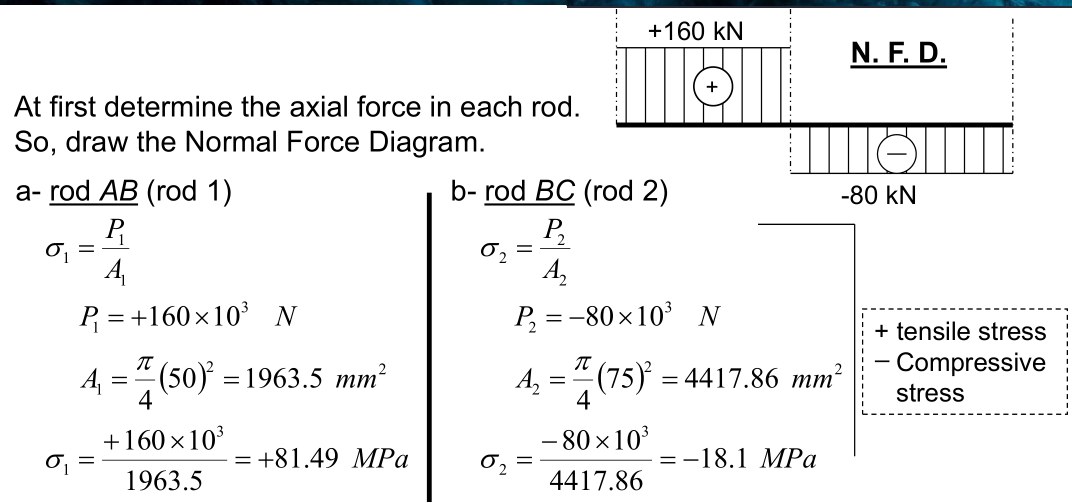
\includegraphics[scale=0.5]{figures/2021-03-30_22-40.png}
\end{sln}
NFD = Normal Force Diagram

\end{document}
